%
\documentclass[12pt,notitlepage]{article}
\usepackage{amssymb}
\usepackage{amsmath}
\usepackage{graphicx}
\usepackage{graphics}
\usepackage{epstopdf}
\usepackage{pdflscape}
\usepackage{subfig}
\usepackage{tabularx}
\usepackage{longtable}
\usepackage{array}
\usepackage{dsfont}
\usepackage{float}
\usepackage{booktabs}
\usepackage{marvosym}
\usepackage{multirow}
\usepackage{pdflscape}
\usepackage[hyphenbreaks]{breakurl}
\usepackage[hyphens]{url}
\usepackage{setspace}
\usepackage{epigraph}
\usepackage{bm}
\usepackage{textcomp}
\usepackage{bbm}
\usepackage{tikz}
\usepackage{siunitx}
\usetikzlibrary{positioning}
\usepackage{afterpage}
\usepackage{lipsum}
\usetikzlibrary{fit}
\tikzset{mynode/.style={draw,text width=1in,align=center}}
\usepackage{verbatim}
\usepackage{amsmath}
\usepackage{setspace}
\usepackage{multibib}
\newcites{online}{References}
\usepackage[round]{natbib}
\usepackage[shortlabels]{enumitem}
\setlength{\epigraphrule}{0pt}

\setcounter{MaxMatrixCols}{10}

\usepackage{natbib,hyperref}
\bibliographystyle{chicago}  

\newcolumntype{C}[1]{>{\centering\let\newline\\\arraybackslash\hspace{0pt}}m{#1}}

\topmargin=-2cm \textheight=24cm \oddsidemargin=-0.5cm
\evensidemargin=0.0cm \textwidth=17.5cm
\usepackage[bottom]{footmisc}
\newtheorem{ass}{Assumption}
\newtheorem{definit}{Definition}
\newtheorem{prop}{Proposition}
\newtheorem{thm}{Theorem}
\newtheorem{lem}{Lemma}
\newtheorem{conj}{Conjecture}
\newtheorem{cor}{Corollary}
\newtheorem{rem}{Remark}
\renewcommand{\thesection}{\arabic{section}}
\renewcommand{\thesubsection}{\arabic{section}.\arabic{subsection}}
\renewcommand{\thesubsubsection}{\arabic{section}.\arabic{subsection}.\arabic{subsubsection}}

\newcommand\independent{\protect\mathpalette{\protect\independenT}{\perp}}
\def\independenT#1#2{\mathrel{\rlap{$#1#2$}\mkern2mu{#1#2}}}

%Figure path
\def \tabroot{tables/}
\def \figroot{figs/}

\usepackage{epsfig,hyperref}

\hypersetup{
    pdftitle={Econometrics and Happiness},    % title
    pdfauthor={Francesco Ruggieri},     % author
    pdfnewwindow=true,      % links in new window
    colorlinks=true,       % false: boxed links; true: colored links
    linkcolor=black,          % color of internal links
    citecolor=blue,        % color of links to bibliography
    filecolor=black,      % color of file links
    urlcolor=blue           % color of external links
}

\begin{document}

\title{The Effect of Learniasdfaadsf ng Econometrics on Student Happiness: \\ Evidence from UChicago\thanks{\noindent I am grateful to Steve Pischke, Owen Zidar, and Eric Zwick for helpful comments.}
	\vspace{0.2cm}
}
\author{
	\textsc{Francesco Ruggieri}\thanks{University of Chicago, Department of Economics. E-mail: \url{ruggieri@uchicago.edu}}\\
}


\date{\today}
\maketitle

\medskip

\begin{abstract}
	The effect of learning Econometrics on quality of life is theoretically ambiguous. On the one hand, it is well-known that studying Econometrics entails large short-term costs, especially due to lengthy assignments and unnecessarily harsh grading by merciless teaching assistants. On the other hand, Econometrics leads students to a more solid understanding of cause-effect relationships, a skill that can be easily transferred to other disciplines and social sciences. This paper investigates the effect of taking an Undergraduate Econometrics class on lifetime happiness. Using administrative data from the University of Chicago Undergraduate Office and leveraging the random assignment of an Econometrics voucher, we show that attending an Econometrics class raises long-term student happiness by 0.4 standard deviations. Our estimates are robust to the inclusion of demographic controls, and a heterogeneity analysis reveals that this positive effect is particularly strong among students who took ECON 21030 in Spring 2020.
\end{abstract}

\setcounter{page}{0}\thispagestyle{empty}
%\baselineskip1.47\baselineskip%
\doublespacing

\newpage

\section{Introduction}

The first paper predicting a positive effect of learning Econometrics on lifetime outcomes is \cite{chinasyndrome}. More recent studies have challenged this prediction (\citealt{acemoglu}, \citealt{polarization}).

\lipsum[1]

\section{Data}

\lipsum[2-5]

\section{Empirical Strategy}

\lipsum[6-9]

\section{Results}

\lipsum[10-13]

\section{Robustness}

\lipsum[14-15]

\section{Conclusion}

\lipsum[16-17]

\newpage

\begin{spacing}{1} 
	\def\bibfont{\small}
	\renewcommand\refname{References}
	\bibliographystyle{chicago}  
	\bibliography{references}
\end{spacing}

\newpage

\section*{Figures}

\begin{figure}[H]
	\begin{center}
		\caption{Congressional District Exposure to Chinese Import Competition (1991-2016)}
		\vspace{-6mm}
		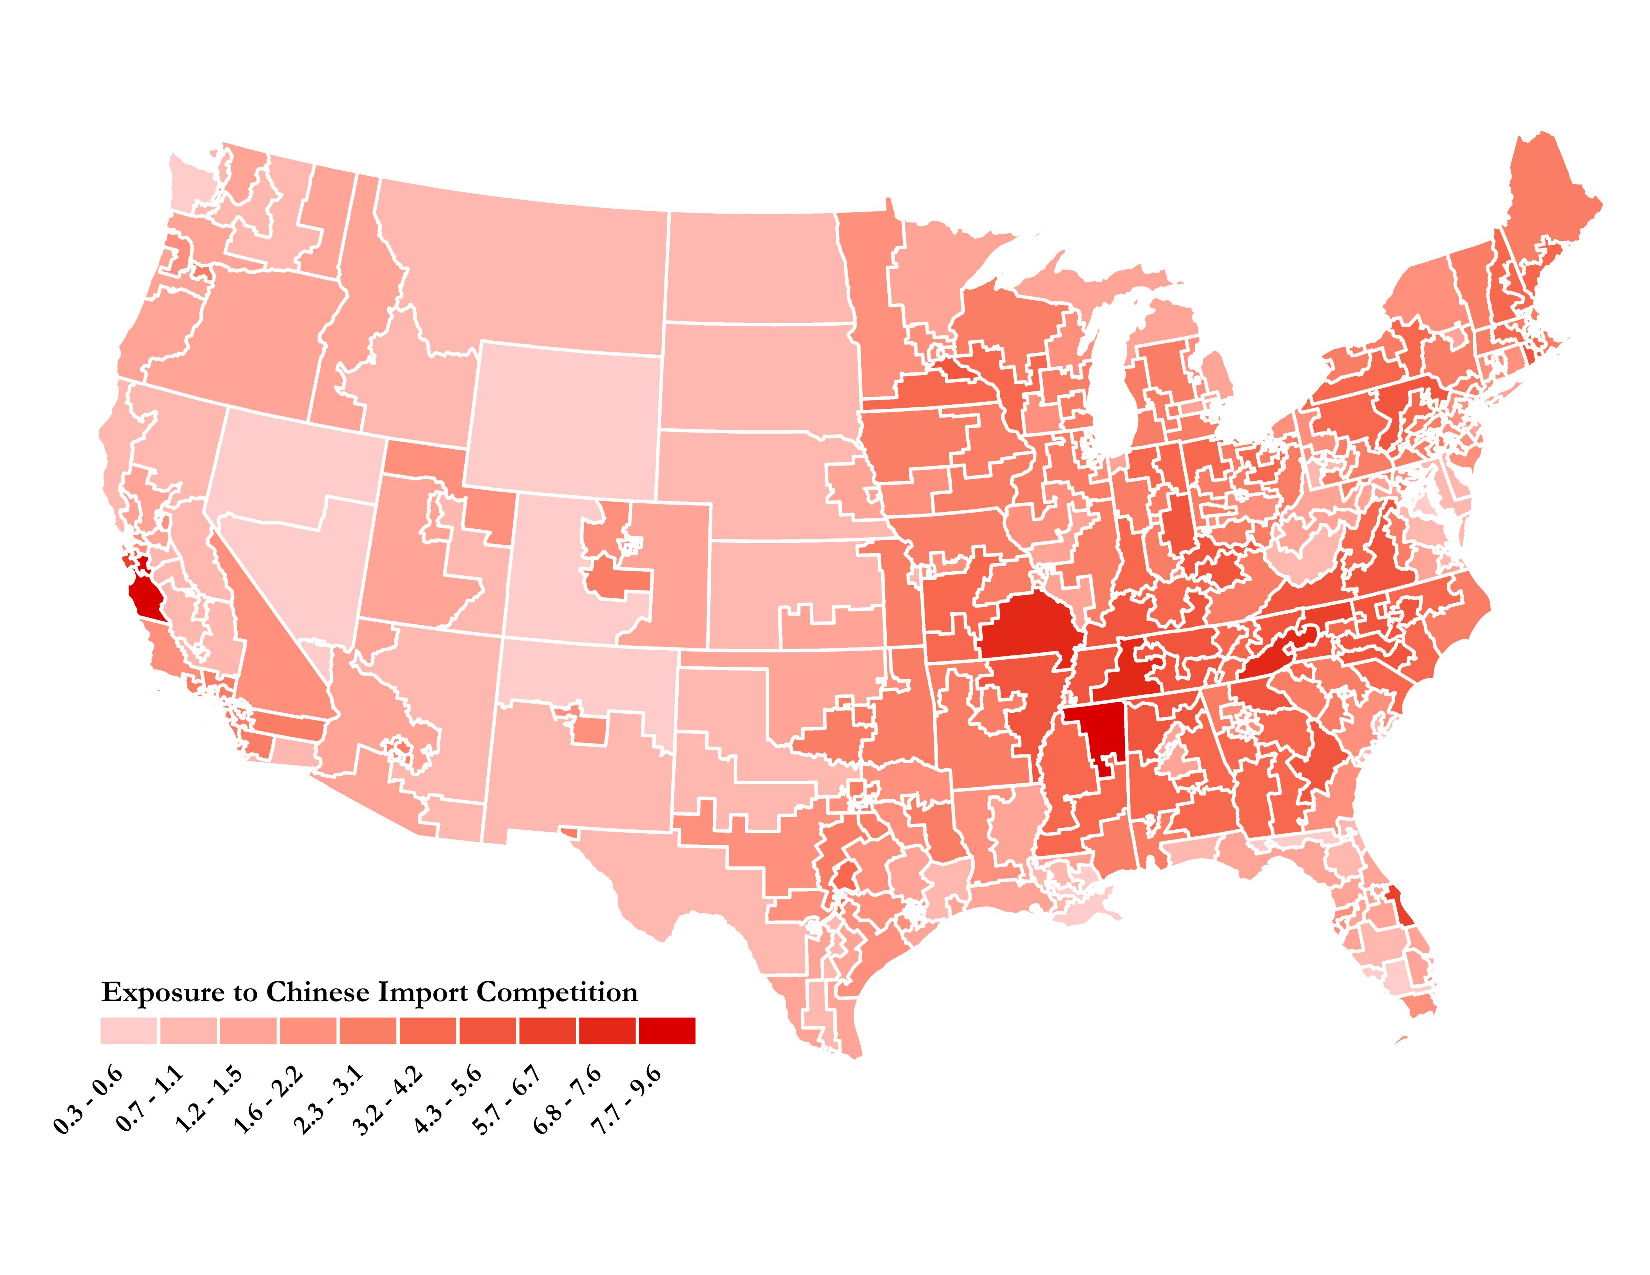
\includegraphics[width=0.8\linewidth]{map_ip_district.pdf}
	\end{center}
\end{figure}
\vspace{-13mm}
\begin{footnotesize}
	\begin{spacing}{1}
		\textsc{Notes}: This figure shows exposure to Chinese import competition by congressional district, as measured by $\Delta IP_{d}$, from 1991 to 2016.
	\end{spacing}
\end{footnotesize}

\newpage

\section*{Tables}

\begin{table}[H]
	\begin{center}
		\caption{Two-Stage Least Squares Estimates}
			\begin{tabular}{lccccc} \hline
 & (1) & (2) & (3) & (4) & (5) \\
 & OLS & F-S & R-F & 2SLS & 2SLS \\ \hline
 &  &  &  &  &  \\
=1 if Took an Econometrics Class & 179.14*** &  &  & 148.10** & 139.37** \\
 & (53.17) &  &  & (60.27) & (57.06) \\
=1 if Received Econometrics Voucher &  & 0.84*** & 125.11** &  &  \\
 &  & (0.01) & (50.94) &  &  \\
 &  &  &  &  &  \\
Observations & 7,983 & 7,983 & 7,983 & 7,983 & 7,983 \\
R-squared & 0.002 & 0.725 & 0.001 & 0.001 & 0.114 \\
 Controls & No & No & No & No & Yes \\ \hline
\end{tabular}

	\end{center}
\end{table}
\vspace{-6mm}
\begin{footnotesize}
	\begin{spacing}{1}
		\textsc{Notes}: This table presents the estimated effects of learning Econometrics on student happiness. Column (1) reports OLS estimates. Column (2) reports estimates of the first-stage equation, in which attendance of an Econometrics class ($D_i$) is regressed onto an indicator that takes the value 1 if a student received an Econometrics voucher ($Z_i$). Column (3) reports reduced-form estimates. In columns (4) through (5), $D_i$ is instrumented with $Z_i$. The model in column (5) controls for race, ethnicity, gender, and student GPA. Robust standard errors in parentheses are clustered at the class level, and *** p$<$0.01, ** p$<$0.05, * p$<$0.1.
	\end{spacing}
\end{footnotesize}

\end{document}